\documentclass[10pt]{beamer}

\usetheme[progressbar=frametitle]{metropolis}
\usepackage{appendixnumberbeamer}

\usepackage{booktabs}
\usepackage[scale=2]{ccicons}

\usepackage{pgfplots}
\usepgfplotslibrary{dateplot}

\usepackage{xspace}
\newcommand{\themename}{\textbf{\textsc{metropolis}}\xspace}

\title{Detecção de artefatos de arritmia utilizando Máquinas de Vetores de Suporte e Coeficientes de Energia Wavelet}
\subtitle{Proposta de TCC}
% \date{\today}
\date{2020}
\author{Gabriel Lechenco Vargas Pereira \\
Cristiano Marcos Agulhari}
\institute{Universidade Tecnológica Federal do Paraná - UTFPR}
% \titlegraphic{\hfill\includegraphics[height=1.5cm]{logo.pdf}} 

\begin{document}
\setbeamertemplate{frame footer}{Universidade Tecnológica Federal do Paraná}

\maketitle

\begin{frame}{Sumário}
  \setbeamertemplate{section in toc}[sections numbered]
  \tableofcontents[hideallsubsections]
\end{frame}

\section{Introdução}

\begin{frame}{Introdução}
    Uma rede pode ser dividida nos seguintes planos:
    \begin{itemize}
        \alert<2>{\item Plano de Dados}
        \alert<2>{\item Plano de Controle}
        \item Plano de Gerenciamento
    \end{itemize}
\end{frame}

\section{Fundamentação Teórica}

\begin{frame}{Eletrocardiograma}
    \begin{figure}[]
      \centering
      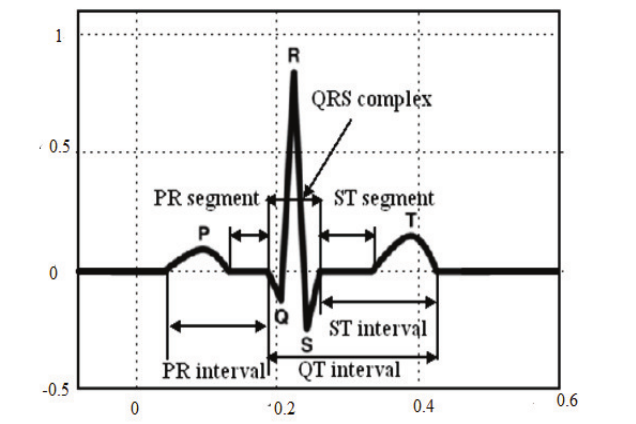
\includegraphics[width=8cm]{images/pqrst.png}
      \caption{Ciclo PQRST \cite{faziludeen_ecg_2013}}
      \label{fig:pqrst}
    \end{figure}
\end{frame}

\begin{frame}{Arritmia}
  A falta de ritmo cardíaco tem ampla influência sobre a saúde do paciente.
  \only<1>{
    \begin{itemize}
      \item Deficiência no transporte e fornecimento de oxigênio.
      \item Podendo acarretar complicações em todo o corpo.
      \item Algumas capazes de levar ao óbito em poucos minutos.
    \end{itemize}
  }

  \only<2>{Imagem taquicardia ventricular}
  
  \only<3>{Imagem fibrilação ventricular}
\end{frame}

\begin{frame}{Máquinas de Vetores de Suporte (SVM)}
    \only<1>{
      Algoritmo de classificação binária que busca encontrar o hiperplano 
      ótimo que seccione o hiperespaço onde os dados se encontram.

      \begin{equation}
        f(x) = \langle w, x \rangle + b = 0
        \nonumber
      \end{equation}

    }
    \only<2>{ 
      \begin{figure}[]
        \centering
        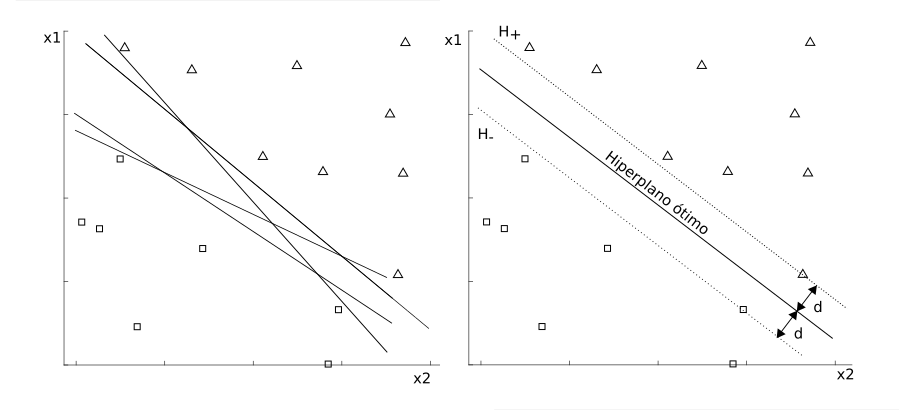
\includegraphics[width=10cm]{images/svmSample.png}
        \caption{Separação de dois planos por um hiperplano ótimo}
        \label{fig:svm}
      \end{figure}
    }
    \only<3,4>{
      Vantagens 
      \begin{itemize}
        \item Otimização de natureza convexa
        \item Apresenta um unico mínimo global para problemas lineares
        \item Consegue bons resultados com poucos exemplos
      \end{itemize}

      \visible<4>{
        Desvantagens
        \begin{itemize}
          \item A princípio resolve apenas problemas lineares
          \item Classificação binária
        \end{itemize}
      }
    }
\end{frame}

\begin{frame}{SVM's e problemas não lineares}
  \only<1>{
    \textbf{Teorema de Cover}
    \begin{quote}
      Dado um problema de classificação de padrões complexo, ao lançá-lo em 
      um espaço com muitas dimensões é mais provável que este seja linearmente 
      separável do que em um espaço com poucas dimensões, desde que o espaço não seja densamente preenchido.
      \cite{haykin_neural_2010}
    \end{quote}
  }
  \only<2>{
    A adição de diferentes kernels possibilita uma maior flexibilidade do algoritmo de
    SVM com uma pequena modificação no problema de otimização.
    \begin{equation}
      f(x) = \langle w, \psi(x) \rangle + b = 0
      \nonumber
    \end{equation}
  }
  \only<3>{
    \begin{figure}
      \centering
      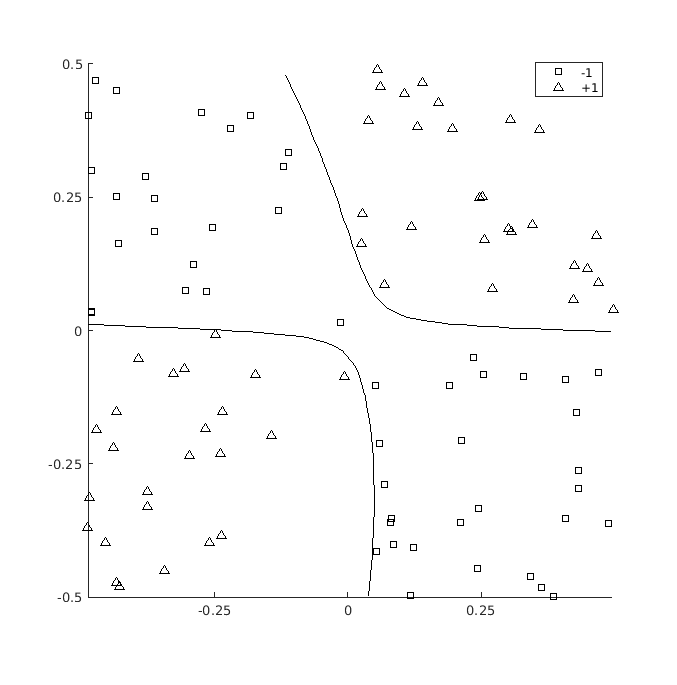
\includegraphics[width=6cm]{images/svmXor.png}
      \caption{SVM utilizando o kernel gaussiano para o problema XOR}
    \end{figure}
  }
\end{frame}

\begin{frame}{SVM's e problemas não binários}

  \only<1>{
    Técnicas pra classificação não binária
    \begin{itemize}
      \item \textit{One Against One} (OAO)
      \item \textit{One Against All} (OAA)
      \item \textit{Directed Acyclic Graph SVM} (DAGSVM)
      \item \textit{Binary Tree of SVM} (BTS)
    \end{itemize}
  }
  \only<2>{\textit{One Against One} (OAO)}
  \only<3>{\textit{One Against All} (OAA)}
  \only<4>{\textit{Directed Acyclic Graph SVM} (DAGSVM)}
  \only<5>{\textit{Binary Tree of SVM} (BTS)}

\end{frame}

\begin{frame}{Wavelet}
    
\end{frame}

\section{Trabalhos Relacionados}

\section{Proposta}

\begin{frame}{Proposta}
    
\end{frame}

\begin{frame}{Pré-processamento}
    
\end{frame}

\begin{frame}{Aprendizado de Máquina}
    
\end{frame}

\begin{frame}{Testes e resultados}
    
\end{frame}

\begin{frame}{Cronograma}
    
\end{frame}

\section{Considerações Finais}

\begin{frame}{Considerações Finais}
    
\end{frame}

{\setbeamercolor{palette primary}{fg=white, bg=mDarkTeal}
\begin{frame}[standout]
  Perguntas?
\end{frame}
}

\appendix


\begin{frame}[allowframebreaks]{References}

  \bibliography{demo}
  \bibliographystyle{abbrv}

\end{frame}

\end{document}
